%!TEX root=../document.tex

\section{Überschrift}
\label{sec:Überschrift}

\subsection{Unterüberschrift}
\label{sec:Unterüberschrift}

\subsubsection{Unterunterüberschrift}
\label{sec:Unterunterüberschrift}

\begin{figure}[!h]
	\begin{center}
		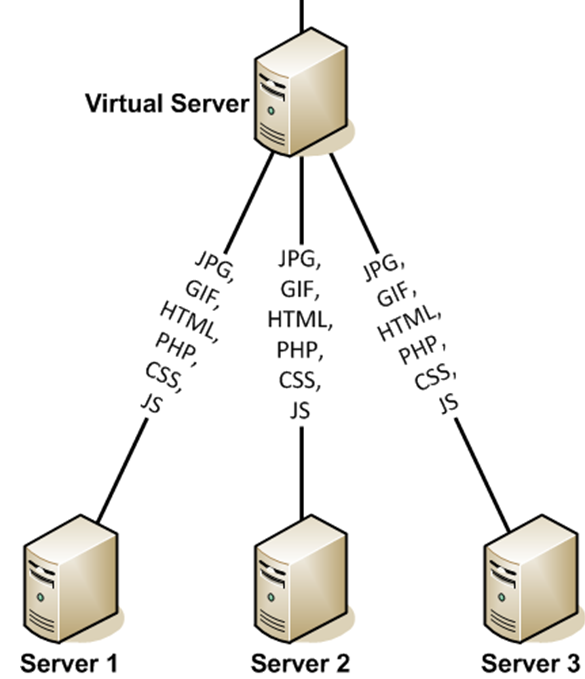
\includegraphics[width=0.5\linewidth]{images/Grafik.png}
		\caption{Ich bin eine Grafik, die eine halbe Seite groß ist und wurde dieser Onlinequelle entnommen \cite{LoadBalancing}}
		\label{Grafik}
	\end{center}
\end{figure}

Wichtig ist, dass du eine entsprechende Größe bei width einträgst und den richtigen Link angibst, Beschriftung und Label fürs Abbildungsverzeichnis nicht vergessen! Zitieren kannst du mit \textbackslash cite\{Kurzbezeichnung der Quelle aus dem BibTex File (references.bib)\}

\textbf{Ich bin fett} \\
Geht mit \textbackslash textbf\{\}

\textit{Ich bin kursiv} \\
Geht mit \textbackslash textit\{\}

\uline{Ich bin unterstrichen} \\
Geht mit \textbackslash uline\{\}

\begin{list}{•}{}
\item Ich bin ein Bullshitpoint
\item Ich auch!
\item Cool!
\end{list}

\begin{list}{-}{}
\item Ich bin ein Element
\item Ich bin auch ein Element
\item Juhuu...
\end{list}

\begin{enumerate}
\item Ich bin die Nummer 1
\item Ich bin die Nummer 2
\item Ich bin die Nummer 3
\end{enumerate}

Tabellen lass ich mal weg, werden wir wahrscheinlich eh nicht brauchen \cite{goossens93}